\section{Durchführung}
\label{sec:Durchführung}

Bei diesem Versuch werden drei Messungen durchgeführt, für die unterschiedliche Versuchsaufbauten verwendet werden. Es wird für alle Messungen ein Diodenlaser
nach Littrow-Aufbau verwendet. Es ist für die Durchführung des Versuches darauf zu achten, diese in einem abgedunkelten Raum durchzuführen. Ebenfalls ist es von
Wichtigkeit, während des gesamten Versuches Schutzbrillen zu tragen.


\subsection{Lasergranulation}

Als erste Messung in diesem Versuch soll mit Hilfe der Lasergranulation der Schwellenstrom des Lasers bestimmt werden. Wenn das Licht des Lasers auf eine Oberfläche
trifft, die Unebenheiten in der Größenordnung der Wellenlänge des Lasers aufweist, dann entstehen an diesen Unebenheiten neue Kugelwellen. Aufgrund der Unebenheit entsteht so
ein zufälliges Interferenzmuster, welches in Form eines körnigen Lichtflecks sichtbar wird. Voraussetzung dafür ist, dass sich der Laser nicht mehr im LED-Bereich befindet und
sein Licht daher ausreichend kohärent ist. Der minimal nötige Strom, um den Laser in diesen Zustand zu bringen wird als Schwellenstrom bezeichnet. Der verwendete Aufbau um diesen
zu bestimmen ist in \autoref{fig:auf1} dargestellt.

\begin{figure}[H]
    \centering
    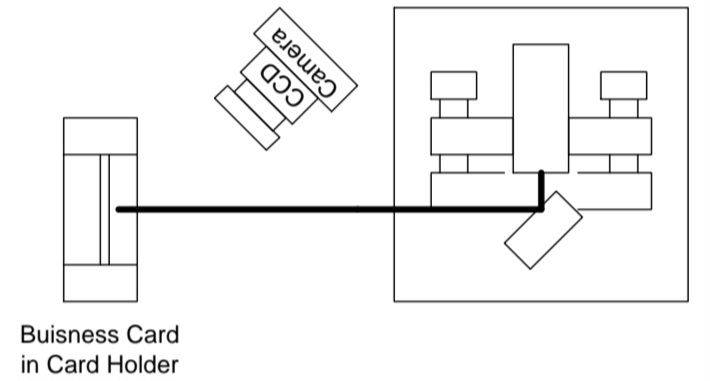
\includegraphics[width=\textwidth]{data/aufbau1.jpg}
    \caption{Der zur Bestimmung des Schwellenstroms verwendete Aufbau \cite{Anleitung60}.}
    \label{fig:auf1}
\end{figure}
\noindent
Das Gitter wird zunächst so eingestellt, dass das Licht des Lasers auf der Detektorkarte sichtbar wird. Es wird dann eine Kamera auf die Detektorkarte ausgerichtet. Im Anschluss
wird der Strom des Lasers langsam erhöht, bis durch die Kamera die ersten Effekte der Lasergranulation sichtbar werden. Diese werden fotografiert und der dafür eingestellte Strom
als Schwellenstrom notiert.


\subsection{Aufnahme der Rubidiumfluoreszenz}

Im nächsten Teil des Versuches soll die Fluoreszenz von Rubidium abgebildet werden. Hierfür wird der in \autoref{fig:auf2} dargestellte Aufbau verwendet.
Dabei wird der Laser mit einem höheren Strom als dem Schwellenstrom betrieben.

\begin{figure}[H]
    \centering
    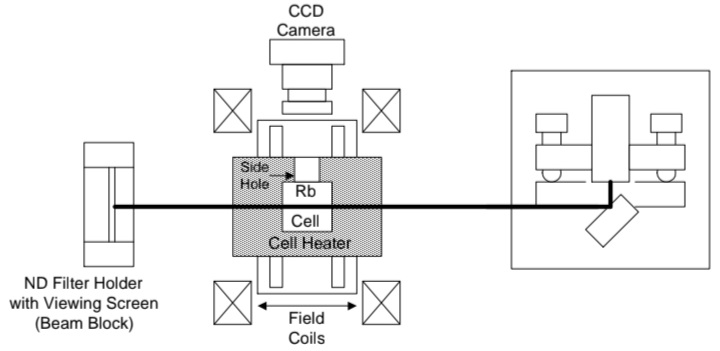
\includegraphics[width=\textwidth]{data/aufbau2.jpg}
    \caption{Der zur Aufnahme der Rubidiumfluoreszenz verwendete Aufbau \cite{Anleitung60}.}
    \label{fig:auf2}
\end{figure}
\noindent
Die Kamera wird transversal zur Rubidiumzelle auf diese gerichtet. Der Laserstrahl wird auf die Rubidiumzelle gerichtet, um das Rubidium anzuregen. Dafür ist jedoch eine
bestimmte Wellenlänge nötig. Diese kann über das winkelverstellbare Gitter und den Strom des Piezokristalls variiert werden. Sobald die Rubidiumfluoreszenz auf der Kamera sichtbar
wird, wird diese fotografiert.

\subsection{Transmissionsspektrum der Rubidiumzelle}

Für die Aufnahme des Transmissionsspektrums der Rubidiumzelle wird vor dieser ein 50/50-Strahlteiler platziert. Beide Strahlen treffen dann auf Photodioden, wobei nur einer von beiden
davor die Rubidiumzelle durchläuft. Die Signale der Photodioden gehen dann an einen Funktionsgenerator. Der finale Aufbau ist in \autoref{fig:auf3} dargestellt.

\begin{figure}[H]
    \centering
    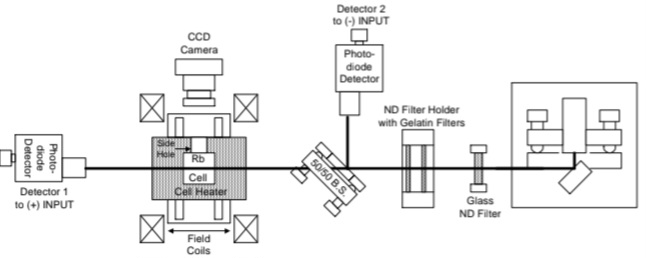
\includegraphics[width=\textwidth]{data/aufbau3.jpg}
    \caption{Der zur Aufnahme des Transmissionsspektrums verwendete Aufbau \cite{Anleitung60}.}
    \label{fig:auf3}
\end{figure}
\noindent
Das Teilen der Strahlen ist wichtig, um den Untergrund herauszufiltern und so den Effekt der Rubidiumzelle zu isolieren. Das Transmissionsspektrum kann dann an einem Oszilloskop
abgelesen und abfotografiert werden.


